% Author: Izaak Neutelings (June, 2018)
\documentclass[border=3pt,tikz]{standalone}
\usepackage{ifthen}
\usepackage{siunitx}
\usepackage{tikz}
\usetikzlibrary{hobby} % for ..
\usetikzlibrary{arrows.meta} % to control arrow size
\tikzset{>={Latex[length=4,width=4]}} % for LaTeX arrow head
\usetikzlibrary{calc,intersections,decorations.markings}
\usepackage{siunitx}
\usepackage{xcolor} % for colored text

\colorlet{mylightblue}{blue!20}
\colorlet{myblue}{blue!50!black}
\colorlet{mydarkblue}{blue!30!black}
\colorlet{mylightred}{red!10}
\colorlet{myred}{red!50!black}
\colorlet{mydarkred}{red!60!black}
\colorlet{mydarkgreen}{green!30!black}

%\tikzstyle{midarr}=[decoration={markings,mark=at position 0.5 with {\arrow{stealth}}},postaction={decorate}]
\tikzset{
    midarr/.style={decoration={markings,mark=at position #1 with {\arrow{stealth}}},postaction={decorate}},
    midarr/.default=0.5
}
\def\tick#1#2{\draw[thick] (#1) ++ (#2:0.03*\ymax) --++ (#2-180:0.06*\ymax)}


\begin{document}


% PHASE TRANSITIONS
    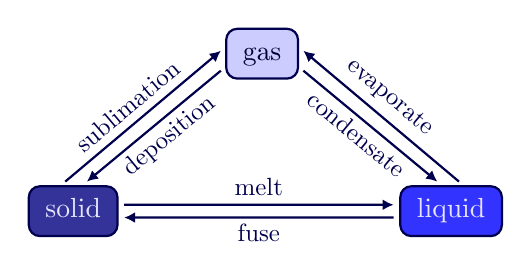
\begin{tikzpicture}[arrow/.style={->,thick,mydarkblue,shorten <=2,shorten >=2},
    box/.style={thick,rounded corners=4,inner xsep=6,inner ysep=3}]
    \message{Phase transitions^^J}

    \node[blue!10!white,draw=mydarkblue,fill=blue!50!gray!80!black,box] (S) at (-2.4,0) {\strut solid};
    \node[blue!10!white,draw=mydarkblue,fill=blue!80!white,box] (L) at (2.4,0) {\strut liquid};
    \node[blue!20!black,draw=mydarkblue,fill=blue!20!white,box] (G) at (0,2) {\strut gas};

    \draw[arrow,->] (S.8) -- (L.173) node[above,midway,scale=0.9] {melt};
    \draw[arrow,->] (L.-173) -- (S.-8) node[below=-1pt,midway,scale=0.9] {fuse};

    \draw[arrow,->] (S.115) -- (G.-190) node[left=2pt,above,midway,sloped,scale=0.9] {sublimation};
    \draw[arrow,->] (G.-160) -- (S.70) node[left=-2pt,below=-1pt,midway,sloped,scale=0.9] {deposition};

    \draw[arrow,->] (L.65) -- (G.10) node[left=2pt,above,midway,sloped,scale=0.9] {evaporate};
    \draw[arrow,->] (G.-20) -- (L.110) node[left=2pt,below=-1pt,midway,sloped,scale=0.9] {condensate};

    \end{tikzpicture}


% PHASE DIAGRAM
    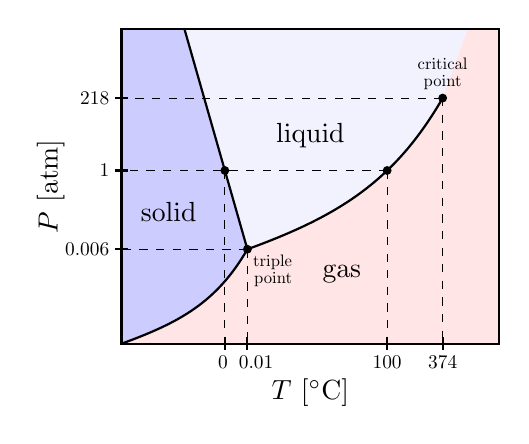
\begin{tikzpicture}[scale=0.4]
        \message{Phase diagrams^^J}

        \def\xtick#1#2{\draw[thick] (#1)++(0,.2) --++ (0,-.4) node[below=-.5pt,scale=0.7] {#2};}
        \def\ytick#1#2{\draw[thick] (#1)++(.2,0) --++ (-.4,0) node[left=-.5pt,scale=0.7] {#2};}

        % COORDINATES
        \coordinate (O) at (0,0);
        \coordinate (N1) at (2,10);
        \coordinate (N2) at (11,10);
        \coordinate (NE) at (12,10);
        \coordinate (NW) at (0,10);
        \coordinate (SE) at (12,0);
        \coordinate (W) at (0,5);
        \coordinate (S) at (6,0);
        \coordinate (C) at (10.2,7.8); % critical
        \coordinate (T) at (4,3); % triple

        % PATHS
        \def\SL{(T) -- (N1)}
        \def\SG{(O) to[out=20,in=-120] (T)}
        \def\LG{(T) to[out=20,in=-120] (C)}
        \def\atm{(0,5.5) -- (12,5.5)}
        \path[name path=SL] \SL;
        \path[name path=LG] \LG;
        \path[name path=atm] \atm;

        % REGIONS
        \fill[mylightblue] \SG -- (N1) -- (NW) -- cycle;
        \fill[blue!5] \LG -- (N2) -- (N1) -- cycle;
        \fill[mylightred] \LG -- (N2) -- (NE) -- (SE) -- \SG -- cycle;
        \node at (1.5,4.2) {solid};
        \node at (7,2.2) {gas};
        \node at (6,6.6) {liquid};

        %% MIXED
        %\shade[top color=mylightblue,bottom color=mylightred,shading angle=70]
        %  (10.4,7.7) -- (11.2,10) -- (10.8,10) -- (10.0,7.7) -- cycle;

        % POINTS
        \fill[black,name intersections={of=SL and atm,by=M}] (M) circle (4pt);
        \fill[black,name intersections={of=LG and atm,by=B}] (B) circle (4pt);
        \fill (T) circle (4pt) node[below right,scale=0.6,align=right] {triple\\[-2pt]point};
        \fill (C) circle (4pt) node[above=1pt,scale=0.6,align=center] {critical\\[-2pt]point};

        % LINES
        \draw[thick] \SG;
        \draw[thick] \LG;
        \draw[thick] \SL;
        \draw[dashed] (M) -- ($(M |- 0,0)$) coordinate (Mx);
        \draw[dashed] (T) -- ($(T |- 0,0)$) coordinate (Tx);
        \draw[dashed] (T) -- ($(T -| 0,0)$) coordinate (Ty);
        \draw[dashed] (B) -- ($(B |- 0,0)$) coordinate (Bx);
        \draw[dashed] (B) -- ($(B -| 0,0)$) coordinate (By);
        \draw[dashed] (C) -- ($(C |- 0,0)$) coordinate (Cx);
        \draw[dashed] (C) -- ($(C -| 0,0)$) coordinate (Cy);

        % AXES
        \draw[thick] (O) rectangle (NE);
        \node[left=17pt,above,rotate=90] at (W) {$P$ [atm]};
        \node[below=9pt] at (S) {$T$ [\si{\degree C}]};
        \xtick{Mx}{\hspace{-2pt}0}
        \xtick{Tx}{\hspace{9pt}0.01}
        \ytick{Ty}{0.006}
        \xtick{Bx}{100}
        \ytick{By}{1}
        \xtick{Cx}{374}
        \ytick{Cy}{218}

    \end{tikzpicture}


% PV diagram - Maxwell construction
    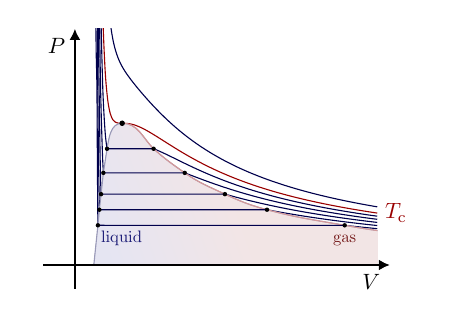
\begin{tikzpicture}
        \message{PV diagram - Maxwell construction^^J}
        \def\xmax{4}
        \def\ymax{3}
        \def\N{110}
        \def\s{0.6}
        \def\A{1.8}
        \def\isotherm#1#2{{ \A*(8*#2)/(3*#1-1) - 3*\A/(#1*#1) }} % reduced equation of state
        \coordinate (C) at (\s,\A);

        % LINE
        \foreach \i/\T/\pe in {0/.75/.28,1/.8/.39,2/.85/.5,3/.9/.65,4/.95/.82,5/1.0/1,6/1.1/1}{

            \begin{scope}
                \clip (-0.15*\xmax,0) rectangle (1.10*\xmax,\ymax);
                \ifthenelse{\i = 5}{
                    \draw[mydarkred,variable=\x,domain=0.36:{.96*\xmax/\s},range=0:1,samples=\N,smooth,name path=isotherm]
                    plot (\s*\x,\isotherm{\x}{\T}) node[mydarkred,right,scale=0.8] {$T_\text{c}$};
                }{
                    \draw[mydarkblue,variable=\x,domain=0.36:{.96*\xmax/\s},range=0:1,samples=\N,smooth,name path=isotherm]
                    plot (\s*\x,\isotherm{\x}{\T});
                }

                \ifthenelse{\i < 5}{ %\lengthtest{\pe pt < 1 pt}
                    \path[name path={pe}] (0,\A*\pe) --++ ({.96*\xmax/\s},0);
                    \path[name intersections={of=isotherm and pe,name=pe\i}];
                }

            \end{scope}
        }

        \begin{scope}
            \clip (0,0) rectangle (.96*\xmax,.96*\ymax);
            \fill[top color=myblue!10,bottom color=myred!10,middle color=myred!10,shading angle=110,
                draw=mydarkblue!40,thin,use Hobby shortcut]
            (.06*\xmax,0) -- (pe0-1) -- (pe1-1) -- (pe2-1) -- (pe3-1) --
            (pe4-1) to[out=80,in=180]
            (C) to[out=0,in=135]
            (pe4-3) to[out=-42,in=145]
            (pe3-3) to[out=-35,in=155]
            (pe2-3) to[out=-25,in=165]
            (pe1-3) to[out=-15,in=170]
            (pe0-3) to[out=-10,in=172]
            (.97*\xmax,.144*\ymax) |- (0,0);
            \draw[mydarkred!40,thin,use Hobby shortcut]
            (C) to[out=0,in=135]
            (pe4-3) to[out=-42,in=145]
            (pe3-3) to[out=-35,in=155]
            (pe2-3) to[out=-25,in=165]
            (pe1-3) to[out=-15,in=170]
            (pe0-3) to[out=-10,in=172]
            (.97*\xmax,.144*\ymax) |- (0,0);
        \end{scope}
        \node[blue!40!black!90,below right=-1,scale=0.6] at (pe0-1) {\strut liquid};
        \node[red!40!black!90,below=-1,scale=0.6] at (pe0-3) {\strut gas};

        % MAXWELL CONSTRUCTION
        \fill (C) circle (1pt);
        \foreach \i in {0,1,2,3,4}{
            \draw[thin,mydarkblue] (pe\i-1) -- (pe\i-3);
            \fill[black] (pe\i-3) circle (.8pt);
            \fill[black] (pe\i-1) circle (.8pt);
        }

        % AXIS
        \draw[->,thick] (0,-0.1*\ymax) -- (0,\ymax)
        node[anchor=north east,inner sep=4,scale=0.8] {$P$};
        \draw[->,thick] (-0.1*\xmax,0) -- (\xmax,0)
        node[anchor=north east,inner sep=4,scale=0.8] {$V$};

    \end{tikzpicture}



\end{document}
